\documentclass{rapport de stage}

\title{Rapport de stage 2A} %Titre du fichier

%----------- Charge la biblio ---------

\addbibresource{biblio.bib} %Import the bibliography file

%----------- Document ---------

\begin{document}

\pagenumbering{roman} % On numerote le début du rapport en chiffres romains

%----------- Informations du rapport ---------

% Lien vers le logo de l'entreprise
\logoentreprise{logos/google.png}
% Nom de l'entreprise
\nomentreprise{Google}

% Titre du rapport
\titre{Titre du rapport}
\intitule{Mémoire de stage de 2ème année}

% Pour le bas de la page
\trigrammemention{TPS}

% Nom de la filière
\filiere{Filière Informatique et réseau}
\master{Science des données et systèmes complexes}

% Votre nom
\eleve{NOM Prénom}

% La promo
\promo{2024}

% L'année universitaire en cours
\annee{2022/2023}

% Les dates du stage
\dates{22/05/2023 - 13/08/2023}

% Le nom et adresse du tuteur école
\tuteurecole{
    \textsc{LAMPERT Thomas} \\
}

% Le nom et adresse du tuteur entreprise
\tuteurentreprise{
    \textsc{VU HIEN Duc} \\
}

%----------- Initialisation -------------------
        
\fairemarges % Afficher les marges
\fairepagedegarde % Créer la page de garde

\justify % La suite du document sera en justifié au carré


%------------ Table des matières ----------------

\tabledematieres % Créer la table de matières

%------------ Corps du rapport ----------------

\pagenumbering{arabic} % On numerote maintenant en chiffres arabes

%------------ Introduction ----------------

\section{Introduction}
Dans le cadre de notre collaboration novatrice avec Hager Group, ce projet d'ingénierie élargit les limites de l'efficacité de l'AFDD (Arc Fault Detection Device) en utilisant les capacités innovantes des réseaux génératifs antagonistes (GAN). La mission que nous avons reçue de Hager Group, un leader mondial dans les solutions électriques, consiste à explorer l'intégration de données synthétiques générées par des GAN afin de renforcer la détection des arcs électriques dans leurs systèmes.

Les GAN, des experts dans le domaine de l'apprentissage profond, permettent de générer des données synthétiques de bonne qualité. Nous visons principalement à exploiter ces progrès technologiques afin d'enrichir les ensembles de données déjà existantes de Hager Group. De cette manière, notre objectif est d'accroître la capacité des systèmes d'AFDD à détecter et à diagnostiquer de manière précise les anomalies dans les systèmes électriques, ce qui contribue à la fiabilité et à la sécurité des stations électriques.
\newpage

%------------ Présentation de l'entreprise ----------------

\section{Présentation du sujet}
\subsection{Hager Group}

Hager Group se positionne en tant que leader mondial dans le domaine des solutions pour les installations électriques dans les secteurs résidentiels, tertiaires et industriels. En offrant une gamme complète, de la distribution d'énergie à la gestion intelligente des bâtiments, en passant par le cheminement de câbles et les dispositifs de sécurité, l'entreprise incarne l'innovation électrique. Dirigée de manière indépendante par les membres de la famille Hager, elle opère depuis son siège à Blieskastel, en Allemagne. Avec 13 000 collaborateurs répartis sur 22 sites dans le monde, Hager Group réalise un chiffre d'affaires de 3,1 milliards d'euros (2023) et exporte ses solutions vers plus de 100 pays. La confiance mondiale témoignée envers Hager Group est le socle de son succès continu.

\subsection{Résumé du projet}

L'objectif principal de ce projet est de concevoir une architecture de type GAN afin d'étendre la base de données du groupe Hager, avec pour finalité d'améliorer la détection des défauts d'arc au sein de leurs installations. Ces données synthétiques seront générées à partir d'une base de données réelle et volumineuse fournie par Hager.

\subsection{GAN}

Les réseaux génératifs antagonistes (GAN) sont une catégorie de modèles d'apprentissage profond extrêmement novateurs. Les GAN, composés d'un générateur et d'un discriminateur, ont été développés dans le but de générer des données synthétiques qui ne sont pas distinguables des données réelles. 


\begin{figure}[h]
    \centering
    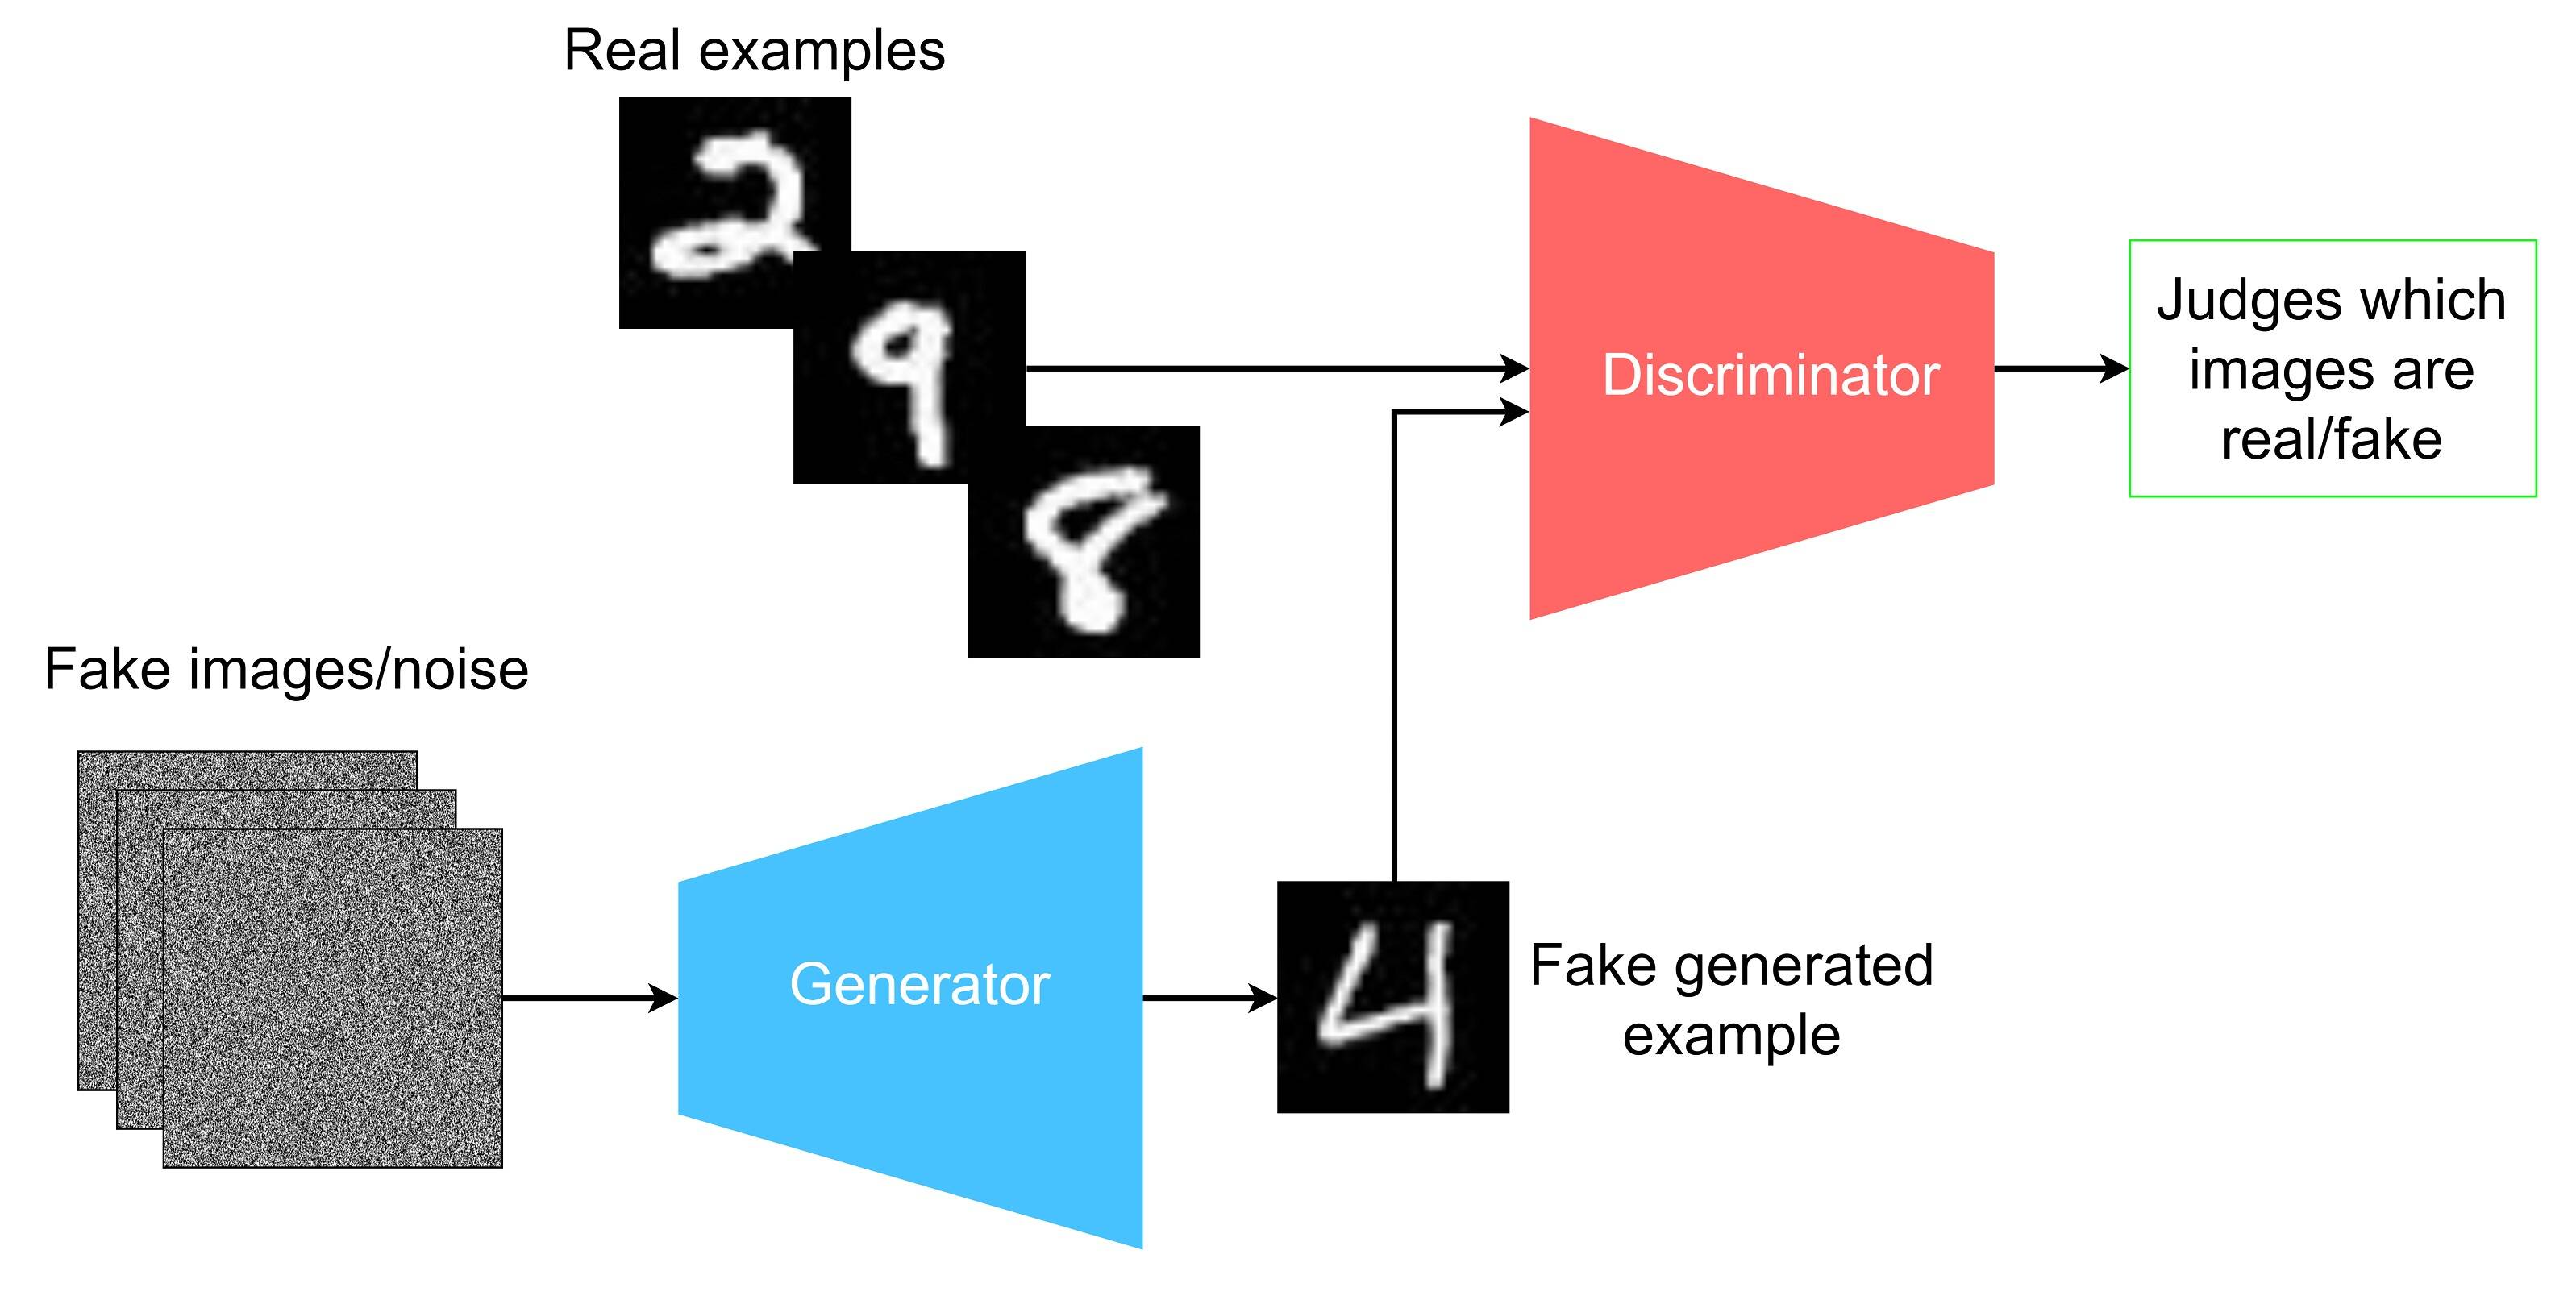
\includegraphics[width=0.6\textwidth]{logos/GANs.jpg}
    \caption{Fonctionnement imagé d'un GAN}
\end{figure}

\newpage

%------------ État de L'art ----------------

\section{État de L'art}
\input{Chapters/EDL}
\newpage

%------------ Diagramme ----------------

\section{Diagramme de Gantt}
\begin{figure}[h]
    \centering
    \includegraphics[width=1\textwidth]{logos/ganttD.png}
    \caption{Diagramme de Gantt}
    \label{fig:enter-label}
\end{figure}
\newpage
%------------ Avancé ----------------

\section{Travail effectué}
\subsection{GAN avec spectrogramme}


\subsubsection{Modèle de base}
Le modèle de générateur initial était conçu avec une structure très simplifiée, comprenant principalement une couche de convolution unique après une transformation linéaire. La configuration de ce modèle se décompose comme suit :

\begin{itemize}
    \item Une couche entièrement connectée qui projette le vecteur latent \( z \) dans un espace de dimensions adaptées pour la mise en forme en image.
    \item Une redimensionnement de la sortie de la couche linéaire pour correspondre à un format d'image tri-dimensionnel, préparant les données pour la convolution.
    \item Une seule couche de convolution pour transformer l'image traitée par la couche précédente, utilisant une fonction d'activation tanh pour normaliser les sorties dans l'intervalle \([-1,1]\).
\end{itemize}

Ce modèle simplifié présente plusieurs limitations :

\paragraph{Manque de profondeur}
Avec une seule couche de convolution, le réseau est limité dans sa capacité à extraire et à recomposer des caractéristiques complexes des données d'entrée

\paragraph{Problèmes de généralisation}
Le modèle souffre également de sous-apprentissage, car les valeurs des pertes du discriminateur et du générateur ne convergent pas. La perte du discriminateur reste très basse, généralement entre 0 et 1, tandis que celle du générateur fluctue considérablement, reflétant la performance variable du réseau de neurones.

\paragraph{Résolution et détails}
Il est également difficile pour le modèle de capturer les détails ; plusieurs couches supplémentaires sont nécessaires pour qu'il puisse générer des images avec une finesse accrue.

\begin{figure}[ht]
    \centering
    \begin{subfigure}[b]{0.45\textwidth}
        
\includegraphics[width=\textwidth]{logos/real_sample.png}
        \caption{Exemple d'image d'entrainement}
        \label{fig:image1}
    \end{subfigure}
    \hfill % Espacement entre les images
    \begin{subfigure}[b]{0.45\textwidth}
        
\includegraphics[width=\textwidth]{logos/generated_samples1.png}
        \caption{Première image générée avec le modèle de base au bout d'une heure d'entraînement.}
        \label{fig:image2}
    \end{subfigure}
    \caption{Images côte à côte}
    \label{fig:images_cote_a_cote}
\end{figure}


\subsubsection{Modèle amélioré}
La deuxième modification majeure concernait l'introduction de couches de convolution supplémentaires dans l'architecture du générateur. Cette modification visait à améliorer la capacité du modèle à capturer et à reproduire des détails plus fins dans les images générées. Les couches ajoutées ont permis une hiérarchisation plus complexe des traits caractéristiques, ce qui a entraîné une augmentation notable de la qualité visuelle des spectrogrammes produits.

\begin{figure}[H]
    \centering
    
\includegraphics[width=0.8\textwidth]{logos/generated_samples2.png}
    \caption{Impact de la modification sur la qualité des images générées}
    \label{fig:mod2}
\end{figure}

Cette amélioration est visible dans les images générées, où les textures et les gradients sont plus naturels et mieux définis par rapport au modèle initial. Cette approche a également contribué à une convergence plus stable des fonctions de perte pendant l'entraînement.


Illustration des changements de performance ou de qualité des résultats.
\begin{figure}[H]
    \centering
    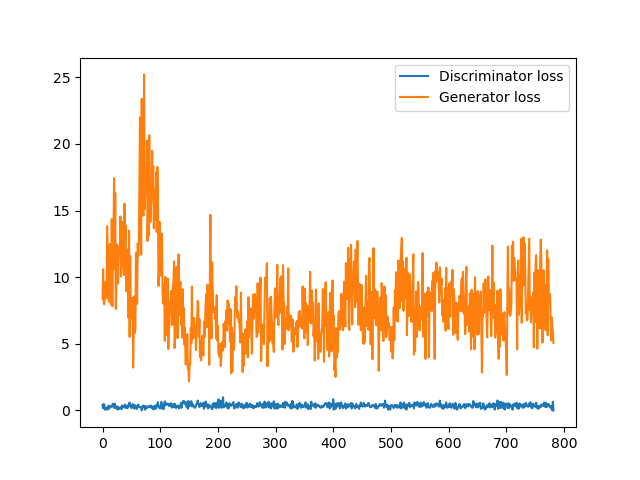
\includegraphics[width=0.4\textwidth]{logos/loss.png}
    \caption{Impact de la Modification 2}
    \label{fig:mod2}
\end{figure}

\subsubsection{Prochaines idées et pistes}
Pour poursuivre l'amélioration de notre modèle GAN pour la génération de spectrogrammes, plusieurs pistes peuvent être envisagées :

\begin{itemize}
    \item \textbf{Augmentation des données :} L'introduction de techniques d'augmentation de données plus variées pourrait aider le modèle à mieux généraliser et à produire des résultats de meilleure qualité sur des données non vues lors de l'entraînement.
    \item \textbf{Optimisation des hyperparamètres :} Un tuning plus fin des hyperparamètres, notamment les taux d'apprentissage et le nombre de couches, pourrait potentiellement améliorer la stabilité et l'efficacité de l'apprentissage.
    \item \textbf{Exploration d'architectures avancées :} L'expérimentation avec des architectures de réseau plus complexes, telles que les GANs conditionnels ou les réseaux adversariaux auto-encodeurs, pourrait ouvrir la voie à des améliorations significatives de la qualité des images.
\end{itemize}

Ces initiatives devraient être guidées par des validations expérimentales continues et des comparaisons rigoureuses pour évaluer leur efficacité réelle dans la production de spectrogrammes réalistes et utiles.

\newpage

%------------ Conclusion ----------------

\section{Conclusion} 
Le projet initié par le groupe Hager offre une opportunité enrichissante pour explorer les applications pratiques de l'intelligence artificielle au sein de notre formation. En traitant un problème concret tel que l'enrichissement de leur base de données pour prévenir les défauts d'arc, ce projet représente une étape cruciale dans notre parcours d'apprentissage. Notre rapport contribue significativement à résoudre les défis réels auxquels font face des industries comme Hager. Nous avons pu élaborer nos premiers modèles et obtenir quelques résultats. Nous pouvons à présent utiliser la puissance de calcul proposée par notre école Télécom Physique Strabourg grâce à l'InnovLab pour effectuer des phases plus importante d'apprentissage. Nous allons aussi pouvoir nous orientier sur conseil de notre tuteur entreprise vers les Transformers. 
\newpage

%------------ Bibliographie ----------------

\section{Bibliographie}
\printbibliography %Prints bibliography
\cite{esteban2017realvalued}
\cite{srinivasan2022timeseries}
\cite{timeGAN}
\cite{article}
\cite{article2}
\newpage


\end{document}